%% nicht vergessen draft raus zu nehmen, um echte Bilder einzubinden und die Problem-Vierecke verschwinden zu lassen
\documentclass[11pt,a4paper,oneside,svgnames]{report}

\usepackage[british]{babel}
\usepackage[utf8]{inputenc}
\usepackage[T1]{fontenc}
\usepackage{ae}
\usepackage{graphicx}
\usepackage{tikz}
\usepackage{kpfonts}
\usepackage[explicit]{titlesec}
\usepackage[acronym,toc,nonumberlist,style=tree]{glossaries}

\makeglossaries

\newglossaryentry{pin}{name=PIN,description={Personal Identification Number},plural=PINs, first={Personal Identification Number (PIN)}}

\newacronym{led}{LED}{light-emitting diode}


\begin{document}

\title{Software Requirements Specifications\\ for\\ Project ``BookExpress''}
\author{Marc A. Harnos\\ {mharnos@gmail.com} \and Joscha Rapp\\ {jraxxo@gmail.com} \and Christian Schulz\\ {crs.s@gmx.net}}
\date{October 2012}
\maketitle
\tableofcontents

\chapter*{Document History}
\begin{tabular}{|l|l|l|l|}
\hline 
Editor(s) & Date & Purpose of Editing & Version \\ 
\hline 
Harnos, Rapp, Schulz & 2012-10-01 & Initial Document Creation & v0.01 \\ 
\hline 
\end{tabular} 

\chapter{Product Purpose}
To handle the addition of new books and the distribution in a better way, "BookExpress" asked us to develop an IT solution to optimize the idle time and labour usage by getting rid of the current, deprecated system. Furthermore one important goal of the software solution is to be very user friendly and easy to use; also there should be remote access implemented, so several customers can access the software at once and distribution partners can access and keep their book stock up to date.
\section{Obligatory Requirements (``must have'')}
The direct connection between the \textbf{customers} and BookExpress shall be implemented by providing a web interface for the customers.\\
\begin{itemize}
\item As each customer already has a unique identifier, the PIN, we will use it as an account name for the login.
\item The web interface has to provide the following features: view catalogue and stock, submit orders, view  the current state of their orders and cancel them (if they haven't been shipped yet)
\item The system has to assign a unique ID to each order
\end{itemize}

The direct connection between the 


\subsection{Book Store}
BLABLABLABLA \gls{pin} BLUB! \gls{led}
\section{Optional Requirements (``nice to have'')}
\section{Non-Requirements (``need to have'')}

\chapter{Product Environment}
The Product takes the orders from the book stores and files them into the system, so that they can be prepared for shipping. For different sized book stores there should be several account types with separate functionality and different options for packaging and ordering. The targeting groups of the software solution are the book store owners, our consumers, the assistants of "BookExpress" and the distribution partners.
\section{Application Area}
\section{User Groups}
\section{Operating Conditions}

\chapter{Product Overview}
The products environmental diagram.

\begin{figure}[h!]
 \begin{center}
  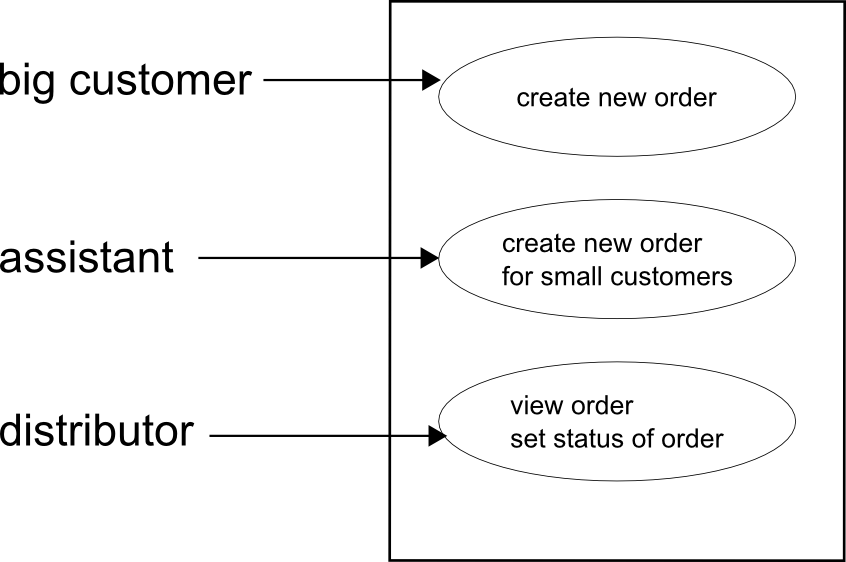
\includegraphics[scale=0.8]{images/umweltdiagramm.png}
 \end{center}
 \caption{The environmental view of the product}
\end{figure}


\chapter{Product Functions}

\section{Internal}
\subsection{Employees of ``BookExpress''}

\hfill \\

\begin{tabular}{p{1.5cm}p{3cm}p{8cm}}
/PF10/	& \textbf{Process}	& Register Publisher or Book Shop (client)\\
		& \textbf{Actor(s)} & BookExpress employee\\
		& \textbf{Category} & \\
		& \textbf{Description}	 & A Book Express employee creates an account for a book shop or publisher after both business partners have signed a contract handling the business relations.\\
		& \textbf{Goal} & The contract partner should have an account to log into the Software. After registration through the Book Express employee, the contract partner will be send a verification and its account information via email.\\
		& \textbf{Preconditions} & Contract signed\\
		& \textbf{Postcondition success} & Successfully created account\\
		& \textbf{Postcondition failure} & Unsuccessful in creating an account\\
		& \textbf{Trigger} & Menu option "register new client" (Software)\\
		& \textbf{Sequence} & Input relevant data and contractor details into the managements system\\
		& & Save the signed contract on the server\\
		& & Register a new client by creating a new ClientID in the database\\
		& & Send verification and account information to the contractor\\
\hfill \\
\end{tabular}


\begin{tabular}{p{1.5cm}p{3cm}p{8cm}}
/PF20/	& \textbf{Process} & Edit client information\\
		& \textbf{Actor(s)} & BookExpress employee\\
		& \textbf{Category} & \\
		& \textbf{Description}	 & The clients data is outdated and needs to be updated\\
		& \textbf{Goal} & Client data is updated\\
		& \textbf{Preconditions} & Client exists in database\\
		& \textbf{Postcondition success} & Client data is updated and a notification mail is sent to the client.\\
		& \textbf{Postcondition failure} & Client data is not updated but rolled back to the previous state. Notification with problem report is shown to the employee.\\
		& \textbf{Trigger} & Menu option "edit client data" (Software)\\
		& \textbf{Sequence} & Menu option "edit client data"\\
		& & Edit specific data\\
		& & Submit edited data to the server\\
\hfill \\
\end{tabular}

\begin{tabular}{p{1.5cm}p{3cm}p{8cm}}
/PF/	& \textbf{Process} & Delete client\\ 
		& \textbf{Actor(s)} & BookExpress Employee\\ 
		& \textbf{Category} & \\
		& \textbf{Description}	 & Client gets deleted due to resignation of the contract\\ 
		& \textbf{Goal} & Delete client from the system\\
		& \textbf{Preconditions} & Client exists in database\\
		& & Contract is being resigned by one of the contractors\\
		& \textbf{Postcondition success} & Client is deleted from the system\\
		& \textbf{Postcondition failure} & Client could not be deleted because of existing orders\\
		& \textbf{Trigger} & Menu option "delete client" (Software)\\
		& \textbf{Sequence} & Choose client\\
		& & Check if client is deletable (i.e. no existing orders)\\
		& & Send notification mail to client\\
		& & Delete client\\
\hfill \\		
\end{tabular}

\begin{tabular}{p{1.5cm}p{3cm}p{8cm}}
	 /PF/	& \textbf{Process} & Client places order (via telephone)\\ 
		& \textbf{Category} & \\
		& \textbf{Actor(s)} & BookExpress employee, client\\ 
		& \textbf{Description}	 & A client orders book via telephone\\ 
		& \textbf{Goal} & Order is placed in an order queue\\
		& \textbf{Preconditions} & Client exists in database\\
		& & Client is authorized\\
		& \textbf{Postcondition success} & Order is placed in an order queue\\
		& \textbf{Postcondition failure} & -\\
		& \textbf{Trigger} & Client initiates order process by calling an BookExpress employee\\
		& & BookExpress employee triggers manual order process\\
		& \textbf{Sequence} & BookExpress employee selects client in Software\\
		& & BookExpress employee enters ordered book into the system\\
		& & Order is placed in order queue\\
		& & Order notification containing detailed report is sent to client\\
\hfill \\
\end{tabular}

\begin{tabular}{p{1.5cm}p{3cm}p{8cm}}
	 /PF/	& \textbf{Process} & Validate order\\ 
		& \textbf{Category} & \\
		& \textbf{Actor(s)} & System\\ 
		& \textbf{Description}	 & Order is checked for validation\\ 
		& \textbf{Goal} & The software checks every order for validation and confirms it to the client. BookExpress knows about every orders validation status.\\
		& \textbf{Preconditions} & Order is in order queue\\
		& \textbf{Postcondition success} & Client receives a confirmation email\\
		& \textbf{Postcondition failure} & Client receives a problem report about invalid order\\
		& \textbf{Trigger} & Order was placed and exists in order queue\\
		& \textbf{Sequence} & System  gathers details and checks whether order is valid or not\\
		& & System sends mail to client\\
\hfill \\
\end{tabular}

\begin{tabular}{p{1.5cm}p{3cm}p{8cm}}
	 /PF/	& \textbf{Process} & Check stock\\ 
		& \textbf{Category} & \\
		& \textbf{Actor(s)} & System/BookExpress employee\\ 
		& \textbf{Description}	 & The system checks whether the amount of books, which the client orders, is available or nearly out of stock.\\ 
		& \textbf{Goal} & Check succeeds\\
		& \textbf{Preconditions} & Order is placed or BookExpress employee initiates check\\
		& \textbf{Postcondition success} & Books which are nearly out of stock get displayed as a list\\
		& \textbf{Postcondition failure} & -\\
		& \textbf{Trigger} & Stock check is initiated\\
		& \textbf{Sequence} & Check \\
\hfill \\
\end{tabular}

\begin{tabular}{p{1.5cm}p{3cm}p{8cm}}
	 /PF/	& \textbf{Process} & Forward order to Logistics\\ 
		& \textbf{Category} & \\
		& \textbf{Actor(s)} & System\\ 
		& \textbf{Description}	 & A validated order gets forwarded to Logistics\\ 
		& \textbf{Goal} & Logistics proceeds processing the order\\
		& \textbf{Preconditions} & Order is valid\\
		& \textbf{Postcondition success} & Logistics processes delivery\\
		& \textbf{Postcondition failure} & Order could not be forwarded to Logistics\\
		& \textbf{Trigger} & Order is validated\\
		& \textbf{Sequence} & Send order information/details to Logistics\\
\hfill \\
\end{tabular}


\section{External}
\subsection{Book Stores (``Clients'')}

\hfill \\

\begin{tabular}{p{1.5cm}p{3cm}p{8cm}}
/PF/	& \textbf{Process} & Client places order (via web interface)\\ 
		& \textbf{Category} & \\
		& \textbf{Actor(s)} & Client\\ 
		& \textbf{Description}	 & Client places an over via the web interface of BookExpress\\ 
		& \textbf{Goal} & Order is placed\\
		& \textbf{Preconditions} & Client is successfully logged into the web interface\\
		& & Connection to BookExpress server is established\\
		& \textbf{Postcondition success} & Order is delivered to BookExpress  and added to the order queue\\
		& \textbf{Postcondition failure} & Order is saved as draft and client gets a notification\\
		& \textbf{Trigger} & Menu Option "create new order" (Web interface)\\
		& \textbf{Sequence} & Client adds books to order (via book search or ISBN)\\
		& & Client specifies amount for every book\\
		& & Client submits order to server\\
		& & Order is in the order queue\\
\hfill \\
\end{tabular}

\begin{tabular}{p{1.5cm}p{3cm}p{8cm}}
	 /PF/	& \textbf{Process} & Search for a book\\ 
		& \textbf{Category} & \\
		& \textbf{Actor(s)} & Client\\ 
		& \textbf{Description}	 & Client searches for a book to add it to his order\\ 
		& \textbf{Goal} & Searching for a book succeeded\\
		& \textbf{Preconditions} & Client is logged into the system\\
		& \textbf{Postcondition success} & Book is being found\\
		& & Display items and options\\
		& \textbf{Postcondition failure} & Book could not be found\\
		& & Display notification\\
		& \textbf{Trigger} & Menu option "find books" (Software)\\
		& \textbf{Sequence} & Enter ISBN/title/author/genre in search bar\\
		& & Hit the "Search"-Button\\
		& & Choose book from list to add it to the order\\
\hfill \\
\end{tabular}

\subsection{Publishers}

\chapter{Product Data}
\section{Customer Data}
\subsection{Book Stores}
\subsection{Publishers}
\section{Order Data}
\section{Internal Data}

\chapter{Product Performance}
\chapter{Quality Requirements}
\begin{table}[h!]
 \begin{tabular}{lllll}
  \hline
  Quality & very good & good & normal & irrelevant \\
  \hline
  Functionality & X & & & \\
  Reliability & X & & & \\
  Usability & & & X & \\
  Efficiency & & X & & \\
  Modifiability & & & X & \\
  Portability & & & & X \\
  \hline
 \end{tabular}
\end{table}

\chapter{User Interface}
\section{Client Application (for clerks)}
\section{Web Interface (for customers)}

\chapter{Non-Functional Requirements}
\chapter{Technical Product Environment}
\section{Software}
\section{Hardware}
\section{Orgware}
\section{Interfaces (product)}

\chapter{Special Requirements for the Development Environment}
\section{Software}
\section{Hardware}
\section{Orgware}
\section{Interfaces (development)}

\chapter{Subproducts and Subsystems}
\section{Server}
\section{Web Interface / Web Service}
\section{Client Application}

\chapter{Additional Specifications and Stipulations}
\chapter{Appendices}
\printglossaries

\end{document}